\documentclass{article}


\usepackage{arxiv}

\usepackage[utf8]{inputenc} % allow utf-8 input
\usepackage[T1]{fontenc}    % use 8-bit T1 fonts
\usepackage{hyperref}       % hyperlinks
\usepackage{url}            % simple URL typesetting
\usepackage{booktabs}       % professional-quality tables
\usepackage{amsfonts}       % blackboard math symbols
\usepackage{nicefrac}       % compact symbols for 1/2, etc.
\usepackage{microtype}      % microtypography
\usepackage{lipsum}
\usepackage{graphicx}
\usepackage[spanish]{babel}
\graphicspath{ {./images/} }


\title{TP 1.2 - ESTUDIO ECONÓMICO-MATEMÁTICO DE APUESTAS EN LA RULETA}


\author{
 Santiago Cancio \\
  Cátedra de Simulación\\
  Universidad Tecnológica Nacional\\
  Zeballos 1341, Rosario, Santa Fe \\
  \texttt{santiago.cancio96@gmail.com} \\
  %% examples of more authors
   \And
 Nicolás Fierro \\
  Cátedra de Simulación\\
  Universidad Tecnológica Nacional \\
  Zeballos 1341, Rosario, Santa Fe\\
  \texttt{nicofierro1@gmail.com} \\
  %% \AND
  %% Coauthor \\
  %% Affiliation \\
  %% Address \\
  %% \texttt{email} \\
  %% \And
  %% Coauthor \\
  %% Affiliation \\
  %% Address \\
  %% \texttt{email} \\
  %% \And
  %% Coauthor \\
  %% Affiliation \\
  %% Address \\
  %% \texttt{email} \\
}

\begin{document}
\maketitle
\begin{abstract}
El siguiente documento se basa en profundizar el estudio del comportamiento de la ruleta desde el punto de vista del apostador y sus estrategias con el objetivo de desmitificar estadísticamente la verdadera probabilidad de obtener ganancias con un medio ideal, como nuestra ruleta simulada.
\end{abstract}


% keywords can be removed
%\keywords{First keyword \and Second keyword \and More}


\section{Introducción}
Nuestro trabajo consistirá en analizar dos estrategias distintas para apostar a la ruleta, donde probaremos las mismas con dos tipos distintos de capitales, siendo uno de ellos capital acotado, el cual será tomado como el caso realista, y el otro siendo con un capital mucho mayor, el cual tomaremos como el caso ideal. Generaremos gráficos de ambas estrategias para analizar cuando se producen ganancias y cuando se producen pérdidas, viendo de esta manera la variación del flujo de caja a medida que la cantidad de tiradas vaya aumentando.\\

Tanto para los casos tomados con capital ideal o capital acotado, la simulacion sera corrida 10 veces graficando de manera simultanea los resultados, para de esta manera lograr conseguir resultados mas confiables y evitar obtener resultados diferentes de lo esperado solo por tener un resultado particular.\\

La ruleta que se utilizará para la simulación será la ruleta tipo Europea, la cuál tiene lo números del 1 al 36 y el 0.

\begin{center}
    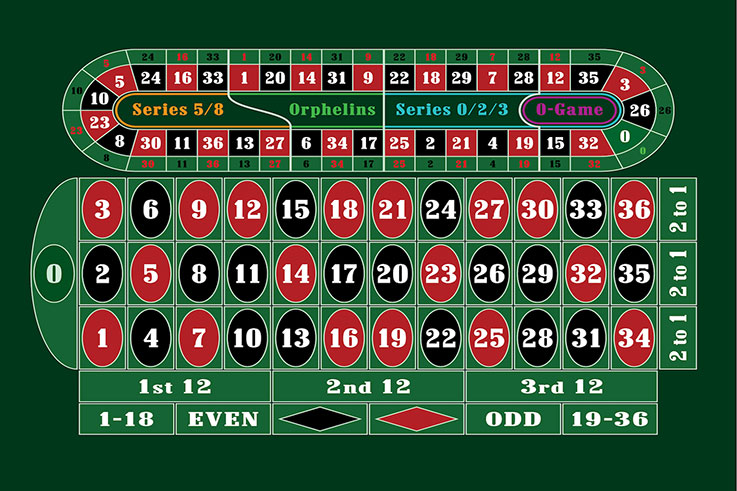
\includegraphics[width=0.5\linewidth]{Ruleta-Europea-Imagen.jpg}
    
    \caption{Figura 1: Ruleta Europea}
\end{center}


\section{Descripción de las estrategias utilizadas}
\label{sec:headings}
En cada corrida realizada, se harán 100 tiradas de la ruleta como máximo, o de lo contrario hasta que el capital acotado con el que cuenta el jugador sea insuficiente para continuar apostando. En todos los casos, las apuestas están definidas de la siguiente manera:
\begin{itemize}
\item Valor de la apuesta: 50
\end{itemize}
\begin{itemize}
\item Capital acotado: 1000
\end{itemize}
\begin{itemize}
\item Capital ideal: 200000
\end{itemize}
A continuación procederemos a nombrar y describir las estrategias que estaremos evaluando.

\subsection{Estrategia Martingala}
Esta estrategia de ruleta nació en Francia en el siglo XVIII y es una de las estrategias de ruleta mas famosas. La misma consiste en apostar una cantidad fija en la apuesta inicial y en caso de pérdida, duplicar esta cantidad apostada hasta que se gane nuestra apuesta. De esta forma, se habrá logrado como beneficio la cantidad que pusimos como nuestra apuesta inicial cuando empezamos a jugar a la ruleta. Se utiliza en las apuestas sencillas como doble o nada: rojo-negro, par-impar, entre otras. A continuacion lo explicaremos mas claramente con un ejemplo muy simple asumiendo que nuestra apuesta inicial es de 1 (nosotros lo evaluaremos con apuestas de 50):\\

\begin{enumerate}
\item  Apostamos 1 a los numeros pares. Si ganamos, repetimos el mismo paso. Si perdemos, vamos al siguiente paso.
\item  Apostamos 2 a los numeros pares (el doble de la anterior). Si ganamos, volvemos al paso 1. Si perdemos, vamos al paso 3.
\item  Apostamos 4 a los numeros pares (el doble del paso 2). De nuevo, si ganamos volvemos a empezar, y si perdemos, seguimos al paso 4.
\item Apostamos 8 a los numeros pares (el doble del paso 2). Igual que en el paso anterior, si ganamos volvemos a empezar, y si perdemos, seguimos al paso 5.
\item Doblamos de nuevo la apuesta: 16. Tanto si se gana como si se pierde, se vuelve al paso 1. Si ganáramos en el último paso, las ganancias ascenderían a 16, mientras que las pérdidas sumarían 1+2+4+8 = 15. Habremos ganado 1, el equivalente a la apuesta inicial.
\end{enumerate}


\subsection{Estrategia de Fibonacci}
Esta es una estrategia para la ruleta creada por Leonardo Pisano Bigollo, al que se le conoció popularmente como Fibonacci. Fue un famoso matemático italiano nacido en el año 1170. Se hizo famoso por descubrir la secuencia de números conocido por su nombre y en que cada número es la suma de los dos números anteriores: 1-1-2-3-5-8-13-21-34-55-89-144-233-377-610.\\

Se puede aplicar como estrategia de ruleta de la siguiente manera: Se comienza apostando una pequeña cantidad a una apuesta simple (negro/rojo, par/impar o 1-18/19-36). Si se pierde, se sigue adelante con la secuencia. Es decir, que si has apostado 1 unidad y pierdes, la siguiente apuesta sería: (0 + 1 = 1) 1 unidad, Si pierdes, apuestas 2 unidades (1+1= 2) siguiendo la sucesión de Fibonacci. Cuando ganes, debes volver dos lugares hacia atrás en la secuencia descrita y apostar esa cantidad. Pero mucho más fácil para entenderlo con este ejemplo con una ronda con apuestas ganadas y perdidas y su desarrollo en la estrategia Fibonacci:
\begin{itemize}
\item Apuesta a los numeros pares, 3, resultado: pierdes.
\item Apuesta a los numeros pares, 3, resultado: pierdes.
\item Apuesta a los numeros pares, 6, resultado: pierdes.
\item Apuesta a los numeros pares, 9, resultado: pierdes.
\item Apuesta a los numeros pares, 15, resultado: ganas.
\item Apuesta a los numeros pares, 6, resultado: pierdes.
\item Apuesta a los numeros pares, 9, resultado: ganas.
\item Apuesta a los numeros pares, 3, resultado: ganas.
\item Apuesta a los numeros pares, 3, resultado: ganas.
\end{itemize}

De esta forma, a pesar de que se ha perdido 5 apuestas por 4 ganadas, se ha logrado obtener beneficios de 3 unidades.

\section{Análisis de resultados}
A continación mostraremos y analizaremos las gráficas dadas a partir de las distintas estrategias simuladas con un capital acotado, que en nuestro caso será de mil unidades.

\subsection{Capital acotado}

\textbf{Martingala:}

\begin{center}
    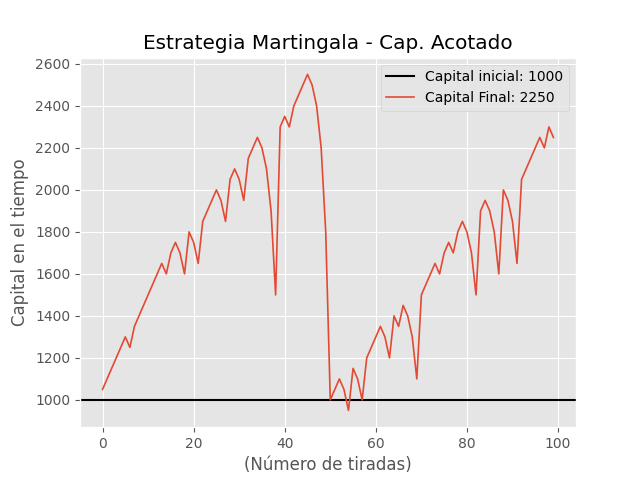
\includegraphics[width=0.7\linewidth]{MG-acotado-1tirada.png}

    \caption{Figura 2: Martingala - Única Corrida}
\end{center}

Como se puede observar en esta gráfica, el jugador comienza con una muy buena racha de victorias con mínimas pérdidas hasta estar cerca de la tirada 40. Un poco antes de llegar a esta tirada el jugador tiene algunas pérdidas considerables, pero luego volvería a ganar incluso más que antes. Al llegar a la tirada 50, el jugador estaría en iguales condiciones en las que empezó, ya que tuvo una considerable baja en su flujo de caja, pero luego comenzaría a ganar nuevamente hasta llegar a tener un capital final de 2250, superando asi por 1250 unidades su capital inicial.

\begin{center}
    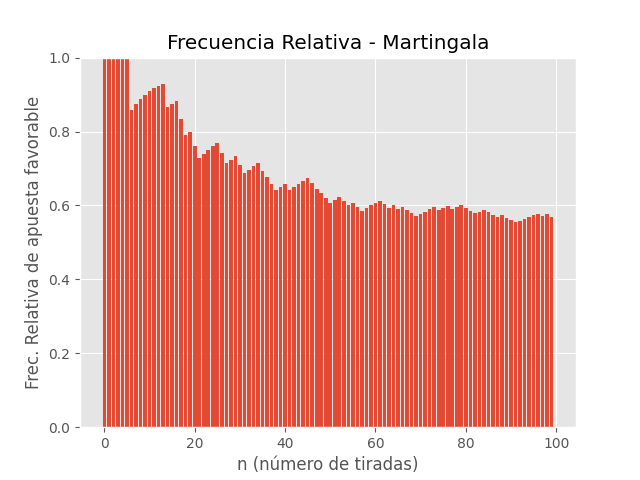
\includegraphics[width=0.7\linewidth]{FreRel-MG.png}
    
    \caption{Figura 3: Frecuencia relativa}
\end{center}


Ahora podemos ver en el gráfico de la frecuencia relativa como varía el valor de esta dependiendo de si se tiene una racha positiva o negativa al comienzo de la sesión y luego a medida que aumentan las tiradas en esta sesión tiende a un valor cercano al 0.6. 


\begin{center}
    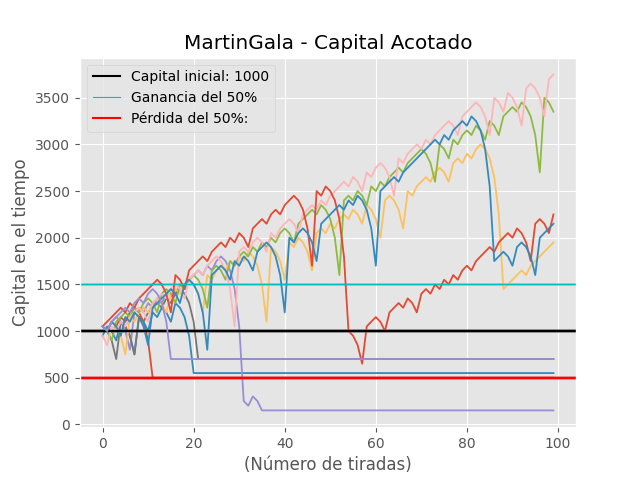
\includegraphics[width=0.7\linewidth]{MG-acotado-multiplestiradas.png}
    
    \caption{Figura 4: Martingala - Múltiples Corridas}
\end{center}

En esta gráfica podemos observar que en la mayoría de los casos el jugador termina teniendo ganancias, incluso más elevadas de lo esperado. Solo en tres de los diez casos simulados el jugador termina con pérdidas suficientes como para no poder continuar apostando.
\\

\textbf{Fibonacci:}

\begin{center}
    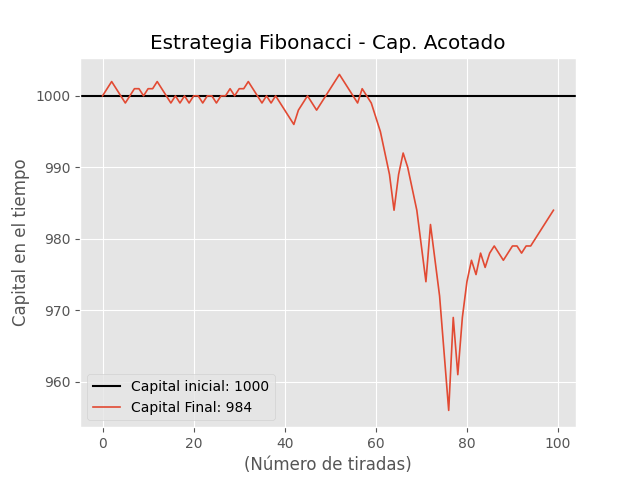
\includegraphics[width=0.7\linewidth]{FIB-acotado-1tirada.png}
    
    \caption{Figura 5: Fibonacci - Única Corrida}
\end{center}

Como podemos observar en esta gráfica, el jugador comienza manteniendose con un valor bastante similar al que tenia apenas había iniciado, pero cerca de la tirada número 60 se puede observar como comienza a haber cada vez mas pérdidas, llegando al pico poco antes de la tirada 80. Afortunádamente para el jugador, unas jugadas más tarde pudo ganar algunas apuestas, recuperando así parte de lo perdido, pero terminando igualmente en una pérdida. Lo bueno de usar esta estrategia es que casi nunca llegamos a apostar cifras muy elevadas, por lo tanto nunca llegaremos a tener pérdidas tan considerables como las podriamos tener utilizando otras estrategias.

\begin{center}
    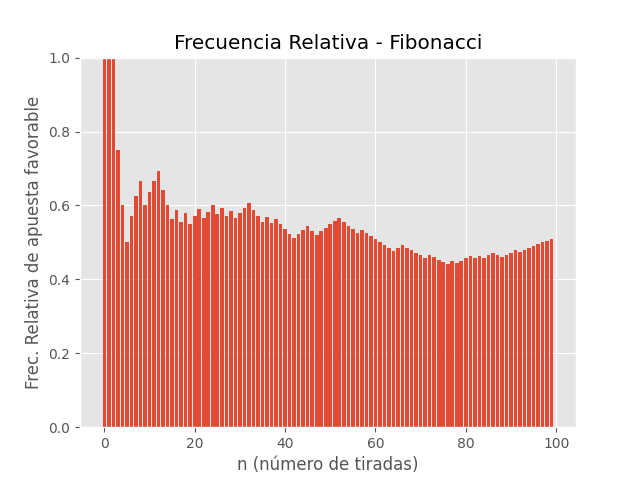
\includegraphics[width=0.7\linewidth]{FreRel-FIB.png}
    
    \caption{Figura 6: Frecuencia relativa}
\end{center}

En este caso podemos observar como varía el valor de la frecuencia relativa, dependiendo de si los resultados fueron positivos o negativos, para llegar a un valor cercano a 0.5 al finalizar las 100 tiradas.

\begin{center}
    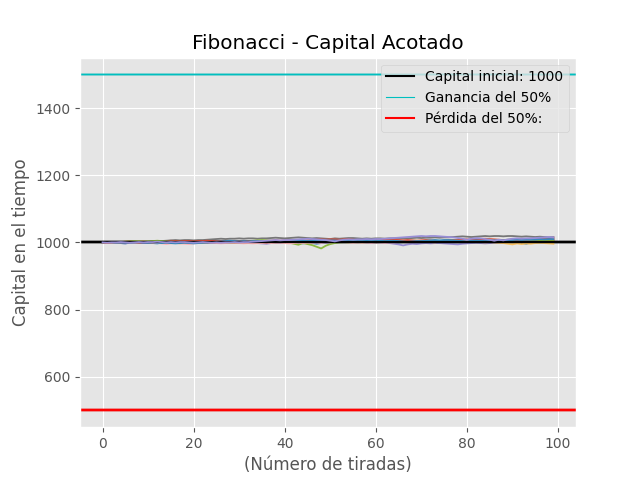
\includegraphics[width=0.7\linewidth]{FIB-acotado-multiplestiradas(1).png}
    
    \caption{Figura 7: Fibonacci - Múltiples Corridas}
\end{center}

\begin{center}
    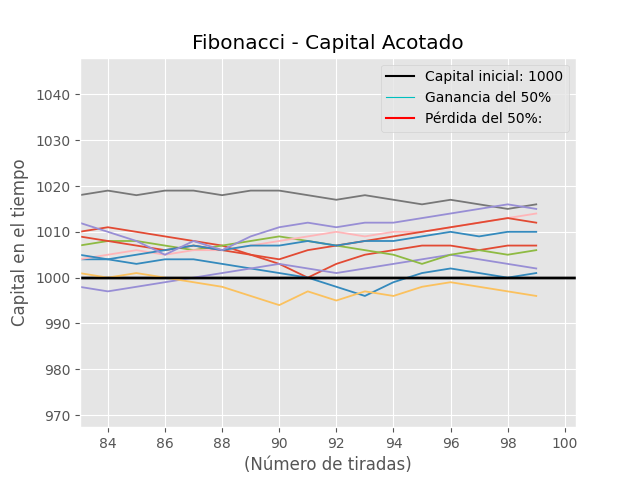
\includegraphics[width=0.7\linewidth]{FIB-acotado-multiplestiradas(2).png}
    
    \caption{Figura 8: Fibonacci - Múltiples Corridas Acercadas}
\end{center}

En este gráfico podemos observar que, al contrario de la gráfica anterior con una sola corrida, en esta en la mayoría de los casos el jugador saldría con un beneficio luego de haber realizado las 100 tiradas. Como mencionamos anteriormente, la pérdida no es muy grande al no apostar demasiado usando esta estrategia, pero tampoco lo es la ganancia, por lo tanto los capitales finales no difieren demasiado del capital inicial.

\textbf{Fibonacci con valores mayores:}

Observando los gráficos de todas las pruebas y corridas que hicimos de la ruleta nos dimos cuenta que la estrategia de Fibonacci se caracterizaba por generar pocas ganancias y pocas pérdidas, ya que a la hora de apostar siguiendo tal sucesión  no se pone en juego una suma de dinero muy grande, sino que si toca una racha ganadora solo se realizan apuestas mínimas. En el caso de una racha perdedora, se iría incrementando la apuesta hasta el caso de ganar, en donde se revierte considerablemente la situación o hasta quedarnos sin dinero.

Debido a esta observación decidimos probar la misma estrategia pero multiplicando por 100 la apuesta según la estrategia anterior. Esto cambia evidentemente el flujo de caja del apostador. Veamos los siguientes gráficos:

\begin{center}
    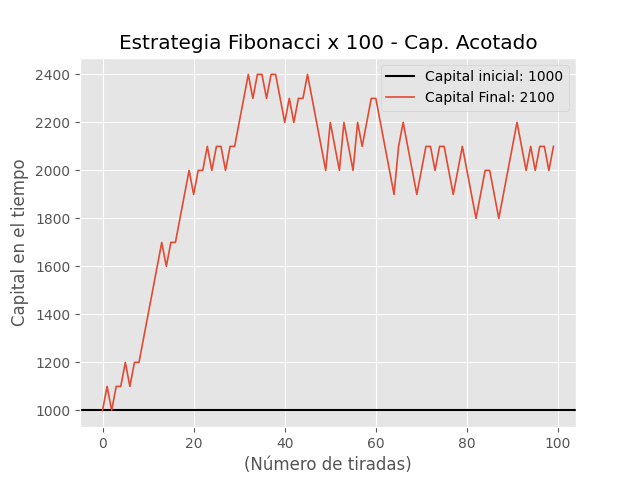
\includegraphics[width=0.7\linewidth]{FIBx100-acotado-1tirada.png}
    
    \caption{Figura 9: Fibonacci Aumentado - Única Corrida}
\end{center}

En esta gráfica se puede notar una gran diferencia si la comparamos con la estrategia de Fibonacci normal. En esta han habido muchas mas ganancias debido a la gran diferencia de montos que se apuestan. Dicho sea esto, de la misma forma que en este caso han habido grandes ganancias, podría haber habido grandes pérdidas.

\begin{center}
    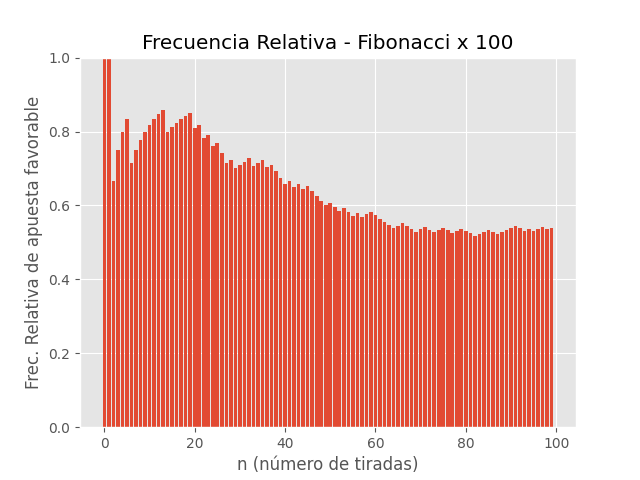
\includegraphics[width=0.7\linewidth]{FreRel-FIBx100.png}
    
    \caption{Figura 10: Frecuencia relativa}
\end{center}

En este gráfico podemos observar la frecuencia relativa de la simulación de la estrategia de Fibonacci modificada, siendo la misma un poco menor a 0.6 al finalizar las 100 tiradas.

\begin{center}
    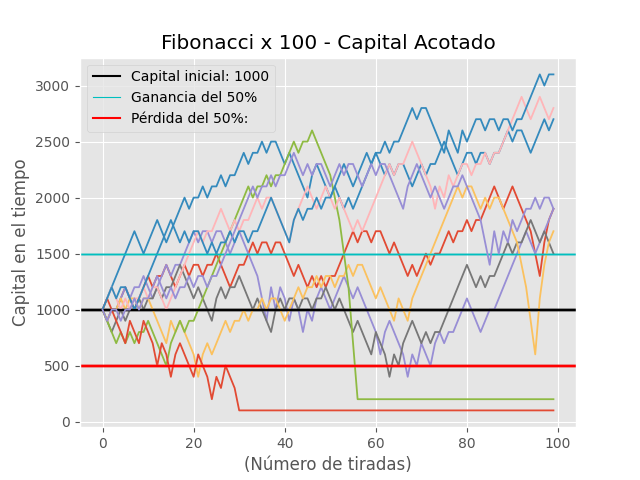
\includegraphics[width=0.7\linewidth]{FIBx100-acotado-multiplestiradas.png}
    
    \caption{Figura 11: Fibonacci Aumentado - Múltiples corridas}
\end{center}

En este gráfico podemos ver que al igual que en la gráfica que incluye solo una corrida, la mayoría de las corridas derivan en una ganancia para el jugador. En este caso, el jugador se quedó en una pérdida total solo en dos ocasiones, mientras que en las otras 8 oportunidades tuvo ganancias importantes.

\subsection{Capital ideal}

A continuación veremos las gráficas de los flujos de caja con cada estrategia utilizada, pero esta vez suponiendo que tenemos un capital de 200.000, el cual consideraremos como ideal.\\

\textbf{Martingala:}

\begin{center}
    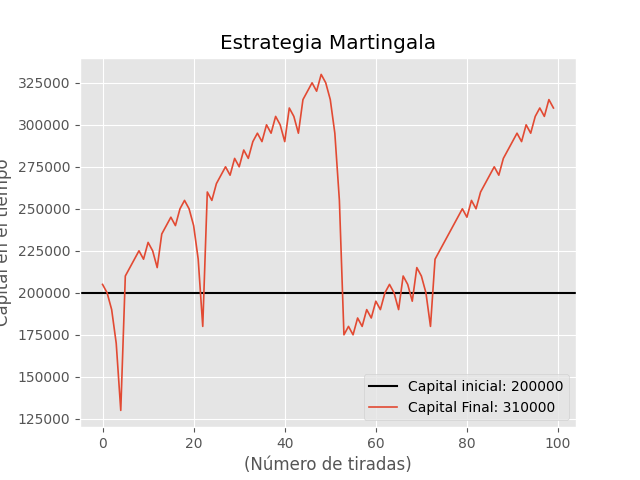
\includegraphics[width=0.7\linewidth]{MG-ideal-1tirada.png}
    
    \caption{Figura 12: Martingala - Única Corrida}
\end{center}

Aquí podemos observar una corrida de la ruleta utilizando la estrategia de Martingala, pero en esta ocasión utilizando un capital ideal de 200000, la cual comienza con una brusca pérdida, pero luego lentamente va recuperando lo perdido. Cerca de la tirada 50 hay otra importante pérdida, pero luego nuevamente comienza a obtener ganancias hasta llegar a salir con un beneficio con respecto al capital inicial al finalizar la tirada número 100.

\begin{center}
    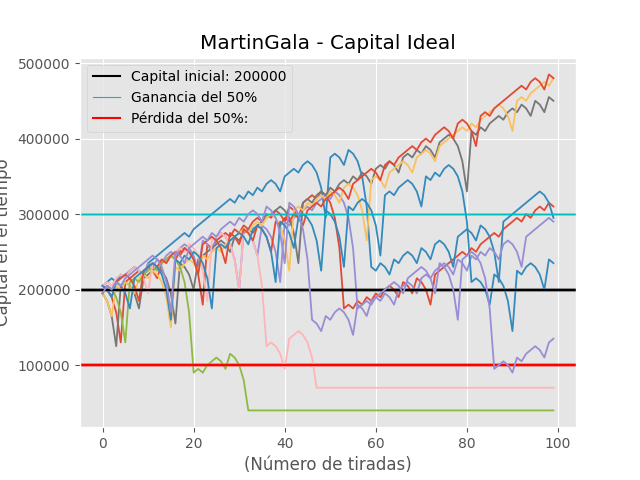
\includegraphics[width=0.7\linewidth]{MG-ideal-multiplestiradas.png}
    
    \caption{Figura 13: Martingala - Múltiples Corridas}
\end{center}

En este caso observamos nuevamente a la estrategia Martingala, pero esta vez con 10 corridas en simultaneo. Al igual que en la gráfica anterior, podemos ver que la mayoría de las veces el jugador termina con un beneficio con respecto al capital con el que había iniciado. Solo en tres ocaciones el jugador termina con pérdidas tras llegar a la tirada 100, y solo 2 de estas 3 tiradas el jugador termina en una pérdida tal que no puede continuar apostando.

\textbf{Fibonacci:}

\begin{center}
    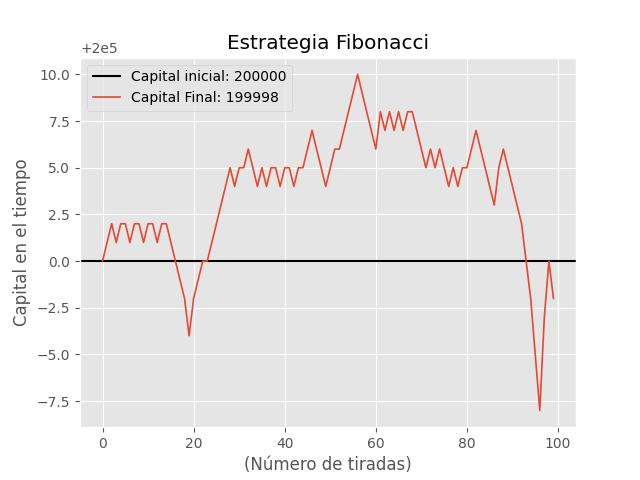
\includegraphics[width=0.7\linewidth]{FIB-ideal-1tirada.png}
    
    \caption{Figura 14: Fibonacci - Única Corrida}
\end{center}

En esta gráfica podemos ver nuevamente a la estrategia de Fibonacci, pero esta vez utilizamos un capital que consideramos como ideal de 200000. En esta ocasión el jugador comienza con una mínima ganancia, para luego tener una brusca pérdida. Luego de eso podemos ver que hay una gran mejora, pero finalmente el jugador termina en una pérdida al llegar a la tirada número 100.


\begin{center}
    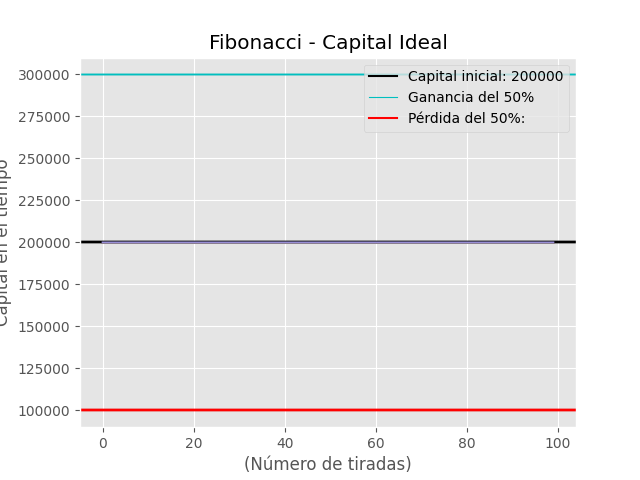
\includegraphics[width=0.7\linewidth]{FIB-ideal-multiplestiradas(1).png}
    
    \caption{Figura 15: Fibonacci - Múltiples Corridas}
\end{center}

\begin{center}
    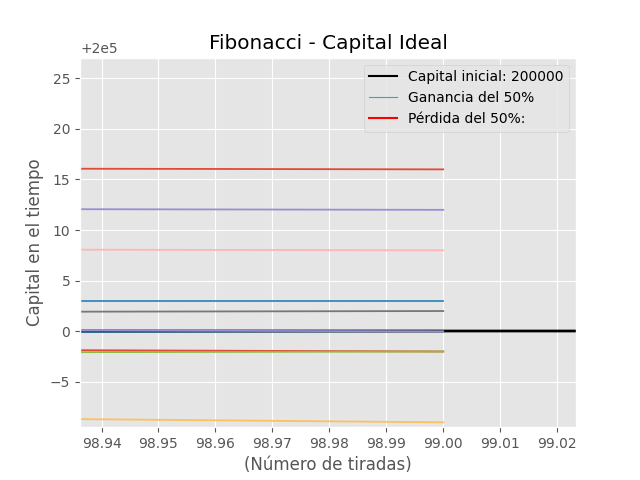
\includegraphics[width=0.7\linewidth]{FIB-ideal-multiplestiradas(2).png}
    
    \caption{Figura 16: Fibonacci - Múltiples Corridas Acercado}
\end{center}


Observando el comportamiento de la estrategia de Fibonacci aplicada con un capital ideal, entendemos que es una estrategia que no es adecuada en el caso de querer ganar dinero rápido sino al contrario. En todos los casos, la estrategia se mantiene constante en pérdidas y ganancias, y al observar las múltiples corridas de la ruleta las ganancias son despreciables en consideración con el capital ideal. Sin embargo en 10 corridas simuladas, se obtienen beneficios en 5 de ellas. 


\textbf{Fibonacci x 100:}

\begin{center}
    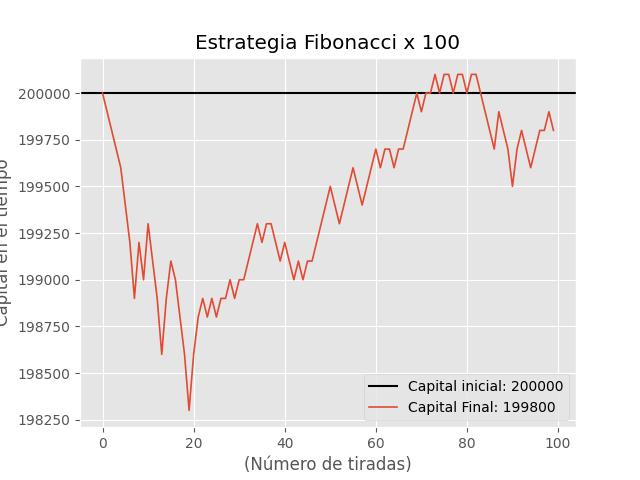
\includegraphics[width=0.7\linewidth]{FIBx100-ideal-1tirada.png}
    
    \caption{Figura 17: Fibonacci Aumentado - Única Corrida}
\end{center}

En esta gráfica podemos observar la estrategia de Fibonacci, pero asumiendo que usamos valores más grandes para las apuestas, por lo que las ganancias y las pérdidas son más pronunciadas. En este caso hay una clara mayoría de pérdidas. Aunque en un momento parece generar ganancias, al finalizar las 100 tiradas hay una pérdida, pero la misma no es tan grande.

\begin{center}
    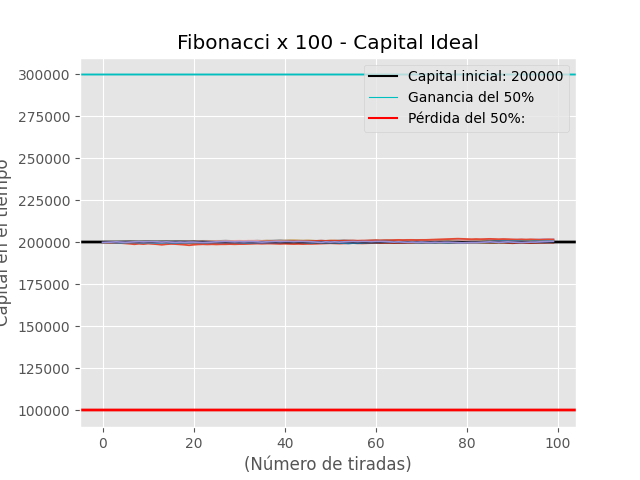
\includegraphics[width=0.7\linewidth]{FIBx100-ideal-multiplestiradas(1).png}
    
    \caption{Figura 18: Fibonacci - Múltiples Tiradas}
\end{center}

\begin{center}
    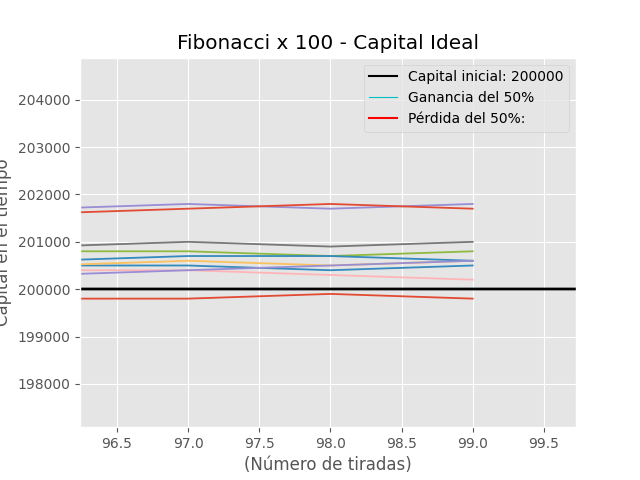
\includegraphics[width=0.7\linewidth]{FIBx100-ideal-multiplestiradas(2).png}
    
    \caption{Figura 19: Fibonacci - Múltiples Tiradas Acercado}
\end{center}

En estas gráficas podemos observar múltiples corridas de la simulación de la estrategia de Fibonacci, nuevamente asumiendo que podemos tomar valores mayores. En este caso, al contrario de la gráfica en la que solo hicimos una corrida, la mayoría de las corridas terminan en una buena ganancia para el jugador, mientras que solo una le genera pérdidas al mismo.

\section{Conclusión}
A través de los análisis que hemos realizado, y gracias a las gráficas expuestas, hemos llegado a la conclusión de que en la mayoría de las ocasiones tanto las estrategias de Martingala como la de Fibonacci o la de Fibonacci con apuestas más grandes, conducen tanto a ganancias como a pérdidas en las distintas corridas que realizamos, lo que hemos notado es que en las ocasiones que tenemos un capital acotado, una vez que hay una gran pérdida es muy difícil poder continuar jugando, mientras que cuando poseemos un capital ideal es más fácil poder remontar la situación y aún así continuar apostando.\\
Esto ha sido lo opuesto a lo que nosotros esperabamos, ya que  esperábamos que a largo plazo todas las estrategias generaran pérdidas. Sin embargo, aunque no todas las corridas hayan generado pérdidas en cuanto al capital inicial, sólo hemos simulado 10 corridas, si se piensa a largo plazo y la cantidad de apostadores que pasan por una ruleta queda demostrado que por probabilidades y matemática que el casino siempre va a obtener un porcentaje de ganancias de las apuestas de la gente dependiendo la jugada que realice y que los números no están a favor del apostador.
Hay un punto que hay que tener en cuenta a la hora de jugar en apuestas de '50 - 50' en la ruleta europea: el número 0, el cuál no se considera número par ni tampoco impar, no se considera color rojo ni negro, sino que es verde, por lo cual no se tiene una probabilidad del 50\% de ganar sino que la probabilidad es del 18/37, mientras que la probabilidad de perder es de 19/37 por lo que el casino tiene un margen del 1,35\% de tus apuestas.
Otro factor importante es que la probabilidad de que salga un número o apuesta simple es totalmente independiente al resultado anterior. 


 


\begin{thebibliography}{1}

\bibitem{Estrategias}
Estrategia Martingala y Fibonacci:
\newblock https://blog.sportium.es/3-simples-estrategias-para-ganar-en-la-ruleta-que-cualquiera-puede-intentar/

\bibitem{Matplotlib}
Librería Matplotlib:
\newblock https://matplotlib.org/

\end{thebibliography}


\end{document}
